%
% This document is available under the Creative Commons Attribution-ShareAlike
% License; additional terms may apply. See
%   * http://creativecommons.org/licenses/by-sa/3.0/
%   * http://creativecommons.org/licenses/by-sa/3.0/legalcode
%
% Copyright 2010 Jérôme Pouiller <jezz@sysmic.org>
%

\part{Gestion de la mémoire utilisateur}

{
\setbeamertemplate{background canvas}{}
\begin{frame}[plain]
  \partpage
  \begin{textblock}{10}(6,11)
    %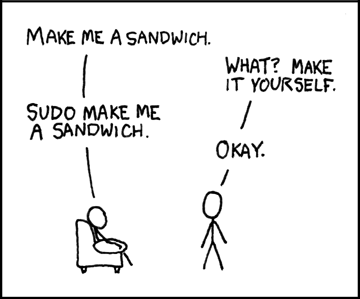
\includegraphics[height=30mm,width=30mm]{sandwich}
    \begin{quote}
      \rmfamily\textit\textbf\color{darkgray}{\large
        ``Knock, knock.\\
        -- Who’s there?\\
        ... very long pause...\\
        -- Java.}
    %  %\vskip3mm\hspace*\fill{\small--- William Shakespeare, Hamlet}
    \end{quote}
  \end{textblock}
\end{frame}
}

\begin{frame}
  \tableofcontents
\end{frame}

\section{Les différents type de mémoire}

\subsection{Les différents segments}

\begin{frame}[fragile=singleslide]{Différents segments}
  \begin{itemize}
  \item \c{.text}: Code \c{r-x}
  \item \c{.data}: Variables globales (et statiques) \c{rw-}
  \item \c{.bss}: Variables globales initialisées à zéro \c{rw-}
  \item \c{.rodata}: Variables globales constantes \c{r--}
  \end{itemize}
  cf. \cmd{objdump -h}
\end{frame}

\subsection{La pile}

\begin{frame}[fragile=singleslide]{La pile}
  \begin{columns}
    \begin{column}{6.5cm}
      \begin{itemize}
      \item Permet d'allouer les variable \emph{auto}.
      \item = Variable locales au fonction
      \item La pile système est composée de \emph{frame}
      \item Chaque appel de fonction ajoute une \emph{frame} à la pile
      \item Deux registres sont utilisé pour la pile:
        \begin{itemize}
        \item Stack Pointer (\c{$sp}): Pointe la tête de la pile
        \item  Frame Pointer  (\c{$fp})  ou Base  stack Pointer  (\c{$bp}):
          Pointe sur (plus ou moins) la base de la frame en cours
        \end{itemize}
      \item On  accède à un variable  locale en lisant  l'adresse \c{$fp + #CONSTANTE}
      \item cf. \cmd{ulimit -s}
      \end{itemize}
    \end{column}
    \begin{column}{4cm}
      \pgfimage[width=5cm]{pics/fig2}
    \end{column}
  \end{columns}
\end{frame}

\begin{frame}{La pile}
  \begin{columns}
    \begin{column}{6cm}
      Lors d'un appel de fonction:
      \begin{itemize}
        \only<1->{
          \item Place les arguments sur la pile (certains arguments peuvent aussi être passé par registre)
        }
        \only<2->{
        \item Sauvegarde du contexte: principalement \c{$ip} (\emph{return address}) et \c{$fp}
        }
        \only<3->{
        \item Affecte \c{$sp} à \c{$fp}, et l'adresse de la fonction à appeller à \c{$ip}
        \item Ajoute la somme de  la taille du contexte  et des variables
          allouées localement à \c{$sp}
        \item Ainsi une allocation locale est très rapide (incrémentation de
          \c{$sp})
        }
      \end{itemize}
    \end{column}
    \begin{column}{6.5cm}
      \begin{overprint}
        \only<1>{
        \pgfimage[width=7cm]{pics/fig3}
        }
        \only<2>{
        \pgfimage[width=7cm]{pics/fig4}
        }
        \only<3>{
        \pgfimage[width=7cm]{pics/fig5}
        }
      \end{overprint}
    \end{column}
  \end{columns}
\end{frame}

  % $sp = $fp
  % $fp = *$fp
  % jmp $sp

  % Sans $fp:
  % $sp = $sp - #FRAME_SIZE
  % jmp $sp

\begin{frame}[fragile=singleslide]{Allocation dynamique sur la pile}
  \begin{itemize}
  \item   Les   fonctions   avec   un  nombre   variable   d'arguments
    (\emph{variadic functions}, cf  \man{va\_arg(3)}) ont une taille de
    frame variable en fonction du nombre d'arguments.
  \item  Il  est  possible   d'allouer  dynamiquement  de  la  mémoire
    supplémentaire sur la frame courante: \man{alloca(3)}
  \item C'est ainsi que sont implémentés des choses du genre
    \begin{lstlisting}
void f(int i) {
   char t[i];
}
    \end{lstlisting}
  \end{itemize}
\end{frame}

\begin{frame}[fragile=singleslide]{\c{omit-frame-pointer}}
  \begin{itemize}
  \item Durant la compilation \cmd{gcc} connait la taille de la frame
  \item Il est  possible de travailler avec \c{$sp}  comme base plutôt
     que \c{$fp}.
    \begin{itemize}
    \item     Au     retour     de     la    fonction,     on     fait
      \c{$sp = $sp - #SIZE_FRAME} au lieu de \c{$sp = $fp}
    \item Cela permet d'économiser un registre
    \item  Permet d'avoir  du code  un peu  plus rapide  en  gérant un
      registre de moins
    \item   Plus   difficile    à   implémenter   car   \c{$sp}   peut
      potentiellement varier
    \item Option \cmd{-fomit-frame-pointer}
    \item Lors  de l'éxecution,  les outils extérieur  (debuggueur) ne
      connaissent  pas la  taille de  la  frame. Ils  ne peuvent  plus
      retrouver  la  base de  la  frame  et  auront des  difficulté  à
      fonctionner.
    \item Depuis la version  6, \c{gdb} possède quelques contournement
      pour deviner la structure de  la pile, mais ca ne fonctionne pas
      toujours.
      \note[item]{Exemple de gdb avec \cmd{-fomit-frame-pointer}}
    \end{itemize}
   \end{itemize}
\end{frame}

\subsection{Le tas}

\begin{frame}[fragile=singleslide]{Le tas}
  \begin{itemize}
  \item Mémoire utilisée par malloc ou new.
  \item  Les  demande  au  Noyau  se font  par  \man{sbrk(2)}  ou  par
    \man{mmap(2)} pour les demandes supérieures ou égale à une page.
  \item malloc ne peut pas utiliser  mmap pour de petits objets car il
    y aurait trop de perte.
  \item  Lors  d'une demande  d'allocation,  \c{malloc} recherche  une
    place dans les pages qu'il a  deja alloué. Si ca n'est pas le cas,
    il appelle \c{sbrk} ou \c{mmap}
  \item malloc ajoute au début  (ou éventuellement à la fin) des blocs
    alloués des information sur la taille du bloc, etc...
  \item Plusieurs algorithme de gestion de \c{malloc}
  \end{itemize}
\end{frame}

\begin{frame}{Liste de blocs}
  Les  liste  de   bloc:  on  utilise  une  liste   chainée  de  blocs
  libre. Lorsqu'on  libére un  bloc, on vérifie  si les  blocs voisins
  sont libres.  On les fusionne si c'était le cas.
  \begin{center}
    \pgfimage[width=10cm]{pics/alloc-freelist}
  \end{center}
  Problème inhérant à cet algorithme: la fragmentation
  \\[2ex]
  Lors  de l'allocation, quatres méthodes.
\end{frame}

\begin{frame}{Liste de blocs}
  \emph{First fit}  On utilise  le premier bloc  assez grand  que l'on
  trouve
  \\
  Exemple (\textbf{A}jout, \textbf{D}elete):
  \begin{center}
    \pgfimage[width=10cm]{pics/alloc-firstfit}
  \end{center}
\end{frame}

\begin{frame}{Liste de blocs}
  \emph{Next  fit} Idem  \emph{First  fit}, mais  on  part du  dernier
  endroit ou a alloué
  \\
  Exemple (\textbf{A}jout, \textbf{D}elete):
  \begin{center}
    \pgfimage[width=10cm]{pics/alloc-nextfit}
  \end{center}
\end{frame}

\begin{frame}{Liste de blocs}
  \emph{Best fit}  On recherche le  bloc disponible de taille  la plus
  proche de  celle nécessaire.  Il s'avère que  cette méthode garantie
  que l'espace inutilisé est petit et donc inutilisable
  \\
  Exemple (\textbf{A}jout, \textbf{D}elete):
  \begin{center}
    \pgfimage[width=10cm]{pics/alloc-bestfit}
  \end{center}
\end{frame}

\begin{frame}{Liste de blocs}
  \emph{Worst  fit}   Utilise  le   plus  gros  bloc   disponible.  En
  comparaison de  \emph{Best fit}, il  ne permet pas d'avoir  des gros
  bloc  aussi important,  en revanche,  il limite  la perte  des petit
  espace.  Paradoxalement, c'est plutot une bonne stratégie.
  \\
  Exemple (\textbf{A}jout, \textbf{D}elete):
  \begin{center}
    \pgfimage[width=10cm]{pics/alloc-worstfit}
  \end{center}
   Problème inhérant à cet algorithme: la fragmentation
\end{frame}

\begin{frame}[fragile=singleslide]{Allocation binomiale}
  Allocation binômiale (buddy system)
  \begin{itemize}
  \item La mémoire disponible est regroupée en bloc de $2^n$ octets
  \item Ainsi, un  bloc d'ordre 2 fait 4 octets,  d'ordre 3, 8 octets,
    etc...
  \item On alloue toujours des bloc d'une taille de puissance de 2
  \item Si  aucun bloc de cette  taille est disponible,  on utilise un
    bloc d'ordre supérieur que l'on divise en deux
  \end{itemize}
  Exemple (\textbf{A}jout, \textbf{D}elete):
  \begin{center}
    \pgfimage[width=8cm]{pics/alloc-buddy}
  \end{center}
\end{frame}

\begin{frame}[fragile=singleslide]{Les pools de mémoires}
  Les pool de mémoires
  \begin{itemize}
  \item  Utilisé dans  les  application allouant  de grandes  quantité
    d'objets identiques
  \item On  crée des pools  de mémoire que  l'on découpe en  espace de
    taille égale
  \item On utilise une simple bitmap pour géré les bloc disponibles
  \item Algorithme le plus rapide et ayant le moins de frgamentation
  \item Principe du slab dans le noyau (\file{/proc/slabinfo})
  \end{itemize}
\end{frame}

\begin{frame}[fragile=singleslide]{\c{brk} vs \c{mmap}}
  Utilisation de \c{brk} ou de \c{mmap}
  \begin{itemize}
  \item \c{brk} garantie  un espace de mémoire continue  ce qui facile
    l'agrandissement
  \item \c{brk} ne permet pas de libérer un bloc au milieu du tas
  \end{itemize}
  Certains algorithme essaie de tirer  profit au maximum de mmap et de
  ne pas allouer de donnée à cheval sur deux pages de mémoires.
\end{frame}

\begin{frame}[fragile=singleslide]{GNU malloc}
  L'implémentation actuelle de  GNU-malloc utilise un mélange de
  ces principes en fontion de la taille du bloc demandé.
  \begin{itemize}
  \item Free-list + Best fit pour les tailles inférieure à 256 octets
  \item buddy-system pour les allocation entre 256o et 256Ko
  \item mmap pour le reste
  \end{itemize}
  %         Reprendre        les        exemples         de        cf:
  % https://umdrive.memphis.edu/blstuart/htdocs/excerpt3.pdf
\end{frame}

\subsection{Détails d'implémentation dans Linux}

\begin{frame}[fragile=singleslide]{Résumé}
  Résumé:
  \begin{itemize}
  \item \emph{File backed memory}
    \begin{itemize}
    \item \c{.text}, \c{.rodata}, \c{.data}
    \item \c{mmap}
    \item Traité comme de la mémoire anonyme si modifié et privée (=Copy-On-Write)
    \end{itemize}
  \item Mémoire anonyme
    \begin{itemize}
    \item \c{.bss}
    \item \c{mmap}
    \item Pile
    \item Tas
    \item Potentielement swapable
    \end{itemize}
  \end{itemize}
\end{frame}

\begin{frame}[fragile=singleslide]{Résumé agencement mémoire}
    \pgfimage[width=8cm]{pics/linuxFlexibleAddressSpaceLayout}
\end{frame}

\begin{frame}[fragile=singleslide]{Fonctionnement Linux}
    \pgfimage[width=8cm]{pics/memoryDescriptorAndMemoryAreas}
\end{frame}

\section{Les garbages collectors}

\subsection{Reference counting}

\begin{frame}[fragile=singleslide]{Reference counters}
 Reference counting
    \begin{itemize}
    \item  Un référence  counter et  un système  qui associe  à chaque
      objet (ou bloc de mémoire) de mémoire un compteur.
    \item Chaque fois que le  pointeur est copié dans une variable, le
      compteur  est incrémenté.  Si la  variable est  écrasée  par une
      nouvelle valeur ou est désallouée, on décrémente le compteur
    \item Si le compteur tombe à zero, on peut désallouer l'objet
    \item  Il est  possible  d'utiliser ce  système  en supplément  de
      l'allocation classique afin de vérifier qu'il n'y a pas d'erreur
      (si  le compteur tombe  à zero,  c'est une  fuite, si  on libère
      alors que le compteur est  supérieur à 1, il y a potentiellement
      un problème)
    \end{itemize}
  \end{frame}

\begin{frame}[fragile=singleslide]{Reference counters}
  Plusieurs manière de l'implémenter:
  \begin{itemize}
  \item En C, on s'interdit les opérateurs d'affectation classiques et
    on  passe  par  des  fonctions qui  effecturons  l'affectation  et
    l'instrumentation.  Très contraingant, difficile de garantir qu'il
    n'y a pas d'autres affectation.  Il n'est pas possible de detecter
    la destruction d'un pointeur qui se trouve sur la pile.
  \item   En  C++,   il   est  possible   de  surcharger   l'opérateur
    d'affectation   pour  rendre  l'opération   transparentes.   Aussi
    appellé   \emph{smart  pointer}   dans   la  literature.    Classe
    \c{shared_ptr}            de            libboost.             (cf.
    \url{http://www.josuttis.com/libbook/cont/countptr.hpp.html})
  \item Dans une  machine virtuelle, ou dans un  langage de script, on
    controle  tous les  accès à  la mémoire,  donc ca  ne pose  pas de
    problème
  \end{itemize}
\end{frame}

\begin{frame}[fragile=singleslide]{Reference counters}
  \emph{Conservative garbage collector}: Il est possible de scanner la
  mémoire  à  la recherche  de  pattern  ressemblant  à des  addresses
  (double mots > 1024).  Il est ainsi possible de retrouver combien de
  pointeur  pointent  sur  chaque  objets. Peuvent  générer  des  faux
  positifs par
  \begin{itemize}
  \item Des pattern qui ressemble à des pointeur
  \item Des pointeurs internes (exemple: heritage d'objets en C++)
  \end{itemize}
  % La  technique  est pas  utilisé comme  garbage
  % collector, mais  plutôt comme outils  d'instrumentation (Dans le
  % noyau Linux: kmemleak)
\end{frame}

\begin{frame}[fragile=singleslide]{Reference counters}
  \begin{itemize}
  \item  Problème 1:  Dans  le cas  de  système multiprocesseurs,  les
    opérations  sur  les pointeur  doivent  être  atomique.  Or  cette
    opértion est relativement lente.
  \item Problème 2: les références circulaires
  \item L'ensemble des objets est un graphe orienté. Il est nécessaire
    de  faire  une  recherche  de  sous-graphe  indépendants.   Si  un
    sousgraphe  n'est référencé  par aucune  variable  globale (.data,
    .rss, etc...) ou locale (pile)
  \item  Il est théoriquement  nécessaire de  faire cette  recherche à
    chaque décrémention  du compteur de référence:  Lent et générateur
    de latence
  \item Lors de la décrémentation  on ajoute l'objet dans la liste des
    objets à vérifier et  on retarde la recherche.
  \end{itemize}
\end{frame}

\begin{frame}[fragile=singleslide]{Reference counters}
  \begin{itemize}
  \item La recherche de sous-graphe se fait alors:
    \begin{itemize}
    \item Lors de l'allocation ou  à un autre moment définit (stop the
      world). Moins de perte de performance, mais toujours problème de
      latence
    \item  Dans  une  thread  séparée  (concurent).   Peut  créer  des
      problème  d'accès concurrents.  Par  forcement possible  sur les
      petit systèmes
    \item Incrémentale,  à chaque déréférencement ou  à chaque période
      de temps fixe, on parcourt une partie du graphe
    \end{itemize}
  \item On peut ajouter des heuristiques sur les objets à scanner. Par
    exemple: commencer par les objets les plus jeunes qui ont surement
    des  durées de  vie plus  courte  que les  vieux objets  (surement
    présent pour toute la durée du vie du programme).
  \end{itemize}
\end{frame}

\begin{frame}[fragile=singleslide]{Autre technique: \emph{tri-color marking}}
  \begin{itemize}
  \item On  arrête le  fonctionnement du programme  à un  moment donné
    (demande d'allocation supplémentaire, etc...).
  \item On utilise trois marques pour les objets:
    \begin{itemize}
    \item blanc: on ne sait pas si l'objet est référencé
    \item gris: l'objet est référencé, mais on a pas encore scanné ses
      dépendence
    \item noir: référencé et analysé
    \end{itemize}
  \end{itemize}
\end{frame}

\begin{frame}[fragile=singleslide]{Autre   technique:  \emph{tri-color
      marking}}
  \begin{itemize}
  \item Au départ, tous les objets sont blancs.
  \item  On marque  gris tous  les objet  accéssible depuis  la racine
    (pile, variables globales).
  \item Pour  chaque element de  l'ensemble gris, on grise  les objets
    référencé et on marque l'objet en noir.
  \item On itère jusqu'à ce que l'ensembel gris soit vide
  \item Tous  les éléments restant dans l'ensemble  blanc peuvent être
    désalloués
  \item On reprend le fonctionnement normal du programme.
  \item  Algorithme \emph{stop  the world}.   Difficultés  pour rendre
    l'algorithme itératif
  \item On peut s'appuyer sur certaines assertion de l'algorithme:
    \begin{itemize}
    \item Un objet noir ne pointe jamais sur un blanc
    \item  Les   objet  vont  toujours   de  blanc,  vers   gris  vers
      noir. Jamais l'inverse.
    \end{itemize}
  \end{itemize}
\end{frame}

\section{Technique de debug mémoire}

\begin{frame}[fragile=singleslide]{dmalloc}
  \begin{itemize}
  \item  Enregistre les  bloc alloué  et les  bloc désalloués.  On est
    capbale de lister les blocs non désalloué en sortie de programme
  \item  Ajout de  garde-fou  avant  et après  les  blocs alloués  par
    malloc. Si lors  de la libération les garde-fous  ont été modifié,
    il y a un problème.
  \item  Ecriture   d'un  pattern  sur  la  mémoire   juste  après  sa
    libération. Permet  de garantir que  les donné lues après  un free
    seront corrompue.
  \item Lors de l'allocation, on vérifie que la mémoire a remplie avec
    le pattern. Si ca n'est pas le cas, une violation d'écriture s'est
    produite entre temps.
  \item  Permet aussi  de garantir  que le  code réinitialise  bien la
    mémoire après l'avoir alloué
  \end{itemize}
\end{frame}

\begin{frame}[fragile=singleslide]{dmalloc}
  \begin{itemize}
  \item Paquet Ubuntu bugué: \url{https://bugs.launchpad.net/ubuntu/+source/dmalloc/+bug/971174}
  %\item \cmd{ wget http://dmalloc.com/releases/dmalloc-5.5.2.tgz}
  %\item \cmd{tar xvzf dmalloc-5.5.2.tgz}
  %\item Suppression des surcharges des fonctions dans \file{malloc.c}
  %\item \cmd{ ./configure && make && sudo make install}
  \item Ajouter \c{#include <dmalloc.h>}
  \begin{lstlisting}
$ gcc -g debug_mem.c -ldmalloc -o debug_mem_dmalloc
$ dmalloc -DV
$ dmalloc -tV
$ dmalloc high -m error-abort -l dmalloc.out
$ echo 123456 | DMALLOC_OPTIONS=debug=0xcb4ed2b,log=dmalloc.out ./debug_mem_dmalloc
$ less dmalloc.out
  \end{lstlisting}
  \end{itemize}
\end{frame}

\begin{frame}[fragile=singleslide]{Libefence, DUMA et kmemcheck}
  \begin{itemize}
  \item Le principe est de s'aider de la MMU pour détecter les erreurs
    d'accès mémoire
  \item  La mémoire est  allouée avec  mmap. On  retire les  droits en
    lecture et en écriture sur le bloc de mémoire alloué.
  \item  A chaque  accès, en  lecture ou  écriture, une  exception est
    déclenché.
  \item Le système récupère la main, log l'accès et vérifie si l'octet
    sur lequel s'effectue l'accès est autorisé
  \item  Permet de détecter  l'erreur dès  qu'elle se  produit (plutot
    qu'à l'allocation suivante)
  \item Permet  de détecter un accès  en lecture sur  une addresse non
    initialisé
  \end{itemize}
\end{frame}

\begin{frame}[fragile=singleslide]{Libefence, DUMA et kmemcheck}
  \begin{lstlisting}
$ gcc -g debug_mem.c -o debug_mem_duma
$ echo 1234 | LD_PRELOAD=/usr/lib/libduma.so.0.0.0 DUMA_FILL=1 DUMA_PROTECT_FREE=1 ./debug_mem_duma
$ gdb -core core debug_mem_duma
  \end{lstlisting}
\end{frame}

\begin{frame}[fragile=singleslide]{Valgrind, kmemleak, Mudflap}
  \begin{itemize}
  \item  Utiliser  un  garbage  collector comme  instrumentation  pour
    vérifier la bonne utilisation de la mémoire
  \item Les différents algorithme de garbage collections s'appliquent
  \item   Kmemcheck:  Instrumentation   avec  un   garbage  collecteur
    conservatif dans le noyau
  \item Valgrind: Machine virtuelle JIT natif/natif
    \begin{itemize}
    \item  Permet   d'instrumenter  tous  les  accès   à  la  mémoire:
      referencement, lecture et ecriture
    \item Permet  de repérer  les fuites ET  les mauvais  accès (comme
      DUMA)
    \item La detection de fuites ou de mauvais accès est immédiate
    \item Plus rapide que DUMA grace à la JIT
    \end{itemize}
  \item Plutôt  que d'instrumenter le code durant  l'éxecution, il est
    possible de l'instrumenter durant la compilation
    \begin{itemize}
    \item Mudflap (compilation avec \cmd{-fmudflap})
    \item Nécessite que toutes les bibliothèques soient instrumentées
    \end{itemize}
  \end{itemize}
\end{frame}

\begin{frame}[fragile=singleslide]{Valgrind}
  \begin{lstlisting}
$ gcc -g debug_mem.c -o debug_mem_valgrind
$ echo 123456 | valgrind --leak-check=yes ./debug_mem_valgrind
  \end{lstlisting}
\end{frame}

\begin{frame}[fragile=singleslide]{Mudflap}
  \begin{lstlisting}
$ sudo apt-get install libmudflap0-4.6-dev
$ gcc -g -fmudflap debug_mem.c -lmudflap  -o debug_mem_mudflap
$ echo 12345 | MUDFLAP_OPTIONS='-help' ./debug_mem_mudflap
$ echo 12345 | MUDFLAP_OPTIONS='-print-leaks -check-initialization' ./debug_mem_mudflap
  \end{lstlisting}
\end{frame}

\section{Communication interprocessus}

\begin{frame}[fragile]{Communication interprocessus}
  Les processus  ayant des espace  mémoire séparés, il  est nécessaire
  d'avoir des systèmes plus évolués pour les faire communiquer:\\
  InterProcessus Communication: IPC.
\end{frame}

\subsection{Mémoire partagée}

\begin{frame}[fragile=singleslide]{La mémoire partagée}
  \begin{itemize}
  \item Utilise  le MMU pour partager  une page de  mémoire entre deux
    processus
  \item dans  cette page de  mémoire, il est possible  d'appliquer les
    mécanisme        de       synchronisation        des       threads
    (\man{pthread\_mutexattr\_getpshared(3)})
  \end{itemize}
\end{frame}

\begin{frame}[fragile]{Mémoire partagée}
  Permet d'implémenter les mécanismes classiques entre processus:
  \begin{itemize}
  \item mutex (réentrant ou non)
  \item rwlock
  \item semaphore
  \item message queues
  \item conditions
  \item barrier/rendez-vous
  \end{itemize}
\end{frame}

\subsection{Cohérence de la mémoire}

\begin{frame}[fragile]{Fonctionnement d'un mutex}
  Nécessite une instruction assembleur  permettant un accès en lecture
  et en écriture  en une instruction: \\
  \texttt{test\_and\_set} affecte le registre d'état en fonction de la
  valeur  du registre  et affecte  la valeur  1 au  registre.  On peut
  développer la fonction \c{lock} à partir de là:
  \begin{lstlisting}
void lock(mutex_t *m) {
  while (test_and_set(m))
    schedule();
}

void unlock(mutex_t *m) {
  m = 0;
  schedule();
}
  \end{lstlisting}
\end{frame}

\begin{frame}[fragile]{Fonctionnement d'un mutex}
  Un peu mieux:
  \begin{lstlisting}
void lock(mutex_t *m) {
  while (test_and_set(m)) {
    this_task.reason = m;
    this_task.state = stop;
    schedule();
  }
}

void unlock(mutex_t *m) {
  m = 0;
  foreach (i in tasks)
    if (i.state == stop && i.reason == m)
      i.state = run;
  schedule();
}
  \end{lstlisting}
\end{frame}

\subsection{Les signaux}

\begin{frame}[fragile=singleslide]{Les signaux}
  \begin{itemize}
  \item Idée issue de l'immitation des interruption sur l'OS
  \item +/- spécifique aux systèmes Posix
  \item L'histoire a rendu l'API un peu bordélique
  \item     \man{sigaction(2)},     \man{signal(7)},    \man{kill(2)},
    \man{kill(1)}, \man{sigqueue(3)}
  \item Il existe 64 signaux sous Linux
  \item Certain  signaux peuvent  être envoyé à  partir de  la console
    (c'est  le   noyau  qui  traduit   les  touches  en   signaux,  cf
    \man{stty(1)})
  \end{itemize}
\end{frame}

\begin{frame}[fragile=singleslide]{Les signaux}
  \begin{itemize}
  \item  Les  signaux  <  32  sont nommés  et  ont  une  signification
    particulière:
    \begin{columns}
      \begin{column}{3cm}
        \begin{itemize}
        \item 1: HUP
        \item 2: INT (\c{^C})
        \item 3: QUIT (\c{^\\})
        \item 4: ILL
        \item 5: TRAP
        \item 6: ABRT
        \item 7: BUS
        \item 8: FPE
        \end{itemize}
      \end{column}
      \begin{column}{3cm}
        \begin{itemize}
        \item 9: KILL
        \item 10: USR1
        \item 11: SEGV
        \item 12: USR2
        \item 13: PIPE
        \item 14: ALRM
        \item 15: TERM
        \item 16: STKFLT
        \end{itemize}
      \end{column}
      \begin{column}{3cm}
        \begin{itemize}
        \item 17: CHLD
        \item 18: CONT
        \item 19: STOP (\c{^Z})
        \item 20: TSTP
        \item 21: TTIN
        \item 22: TTOU
        \item 23: URG
        \item 24: XCPU
        \end{itemize}
      \end{column}
      \begin{column}{3cm}
        \begin{itemize}
        \item 25: XFSZ
        \item 26: VTALRM
        \item 27: PROF
        \item 28: WINCH
        \item 29: POLL
        \item 30: PWR
        \item 31: SYS
        \end{itemize}
      \end{column}
    \end{columns}
    \vspace{2ex}
  \item Il existe  un comportement par défaut pour  chaque signal (fin
    de la tâche, suspension, coredump, ignore)
  \item Il  est possible d'associer ces propres  fonctions aux signaux
    (sauf quelques uns)
  \end{itemize}
\end{frame}

\begin{frame}[fragile=singleslide]{Signaux Temps Réels}
\begin{itemize}
\item Les signaux > 32 sont dit \emph{temps-réel}.
    \begin{itemize}
    \item Plusieurs signaux RT peuvent être en attente
    \item Garantie que les signaux arrivent dans l'ordre dans lesquels
      ils ont été envoyés
    \item Possibilité de passer des valeurs en arguments
    \end{itemize}
  \item Tombent en désuétude. Remplacés par des \emph{file descriptor}:
    \begin{itemize}
    \item \man{signalfd(2)}
    \item \man{eventfd(2)}
    \item \man{timerfd\_create(2)}
    \item \man{inotify(7)}
    \end{itemize}
  \end{itemize}
\end{frame}

\subsection{Les bus logiciels}

\begin{frame}[fragile=singleslide]{Les sockets}
  \begin{itemize}
  \item Généralisation des communications réseaux
  \item Système assez ancien
  \item Mécanisme client/serveur
  \item Le serveur ouvre une socket en écoute
  \item Le client se connecte sur le serveur
  \item  La communication  est  assurée par  des \emph{file  descriptor}
    (\c{read}, \c{write}, etc...)
  \item  Il est  possible  de d'associer  la  socket à  un fichier  (ex:
    \file{/tmp/.X11-unix/X0})
  \end{itemize}
\end{frame}

\begin{frame}[fragile=singleslide]{Les bus logiciels}
  \begin{itemize}
    \item Les socket sont puissants mais manquent d'abstraction
    \item Les \emph{Bus logiciels} offrent les abstraction nécessaires
      \begin{itemize}
        \item Broadcasting d'évènement
        \item Souscription à des évènements/filtrage
        \item Possibilité de passer  des structure complexes comme des
          listes de tailles variables ou des attribut optionnels
        \item   Possibilité   d'interroger   un   processus   distant:
          \emph{Remote Procedure Call (RPC)}
        \end{itemize}
      \item Certains bus peuvent fonctionner à travers un réseau
        \item Certains bus s'appuie sur http et/ou xml
  \end{itemize}
\end{frame}

\begin{frame}[fragile=singleslide]{Les RPC}
  Exemples:
  \begin{itemize}
  \item xml-rpc, soap
  \item corba, dcop, dbus
  \item OLE, COM, DCOM
  \item ømq
  \end{itemize}
\end{frame}
